\section{Experimental Results}
% ── Section 5: Experimental Results ───────────────────────────────────────────
\label{sec:results}

In this section, we present the empirical findings of the proposed framework. We first evaluate a systematic forward purchasing baseline to quantify price differentials across contract horizons. Subsequently, we present the results of Phase 1 (Model and Data Ablation: Single-Seed), which compares the performance of MLP and RecurrentPPO (LSTM) architectures across the eight engineered datasets. Finally, Phase 2 evaluates the effect of algorithmic heuristic adjustments on policy action distributions before progressing to Walk-Forward evaluation.

\subsection{Empirical Baseline Analysis: Forward Price Differentials}
\label{subsec:res_baseline}

Before evaluating DRL policies, we characterise the historical procurement performance of the individual instruments. We simulated a systematic procurement strategy: purchasing a specific forward contract every day and holding it to maturity, comparing the locked price against the eventual SPOT settlement across 1,242 market days (2023--2026).

The analysis reveals a persistent forward--spot price differential in the evaluated Iberian market sample (referred to as the short-horizon forward differential). Systematically purchasing the D1 (day-ahead) contract yields a marginal saving of 2.37\% globally. However, purchasing the D2 (two-days-ahead) contract generates a consistent saving of 13.17\% during the 2025 validation horizon (and 11.95\% across the full 2023--2026 period), with a win-rate of nearly 60\% (with the converged LSTM policy achieving 12.94\%). Conversely, attempting to systematically purchase weekly or monthly contracts results in substantial negative savings (e.g., $-20.72\%$ for M3, and $-31.61\%$ for M4).

The observed D2 differential is consistent with the existence of horizon-dependent forward risk premia documented in electricity derivative markets \cite{huisman2012electricity, woo2001cross, huisman2009electricity}. Electricity derivatives literature shows that forward prices may embed expectations, risk premia and market-specific hedging incentives. The present data are consistent with such an interpretation, but attributing this differential specifically to renewable generators' meteorological uncertainty or zero-price cannibalisation in the SPOT market requires additional evidence on market participants, liquidity and bid-ask prices. In the evaluated historical sample, D2 behaved as a comparatively favourable short-horizon procurement rule, providing positive aggregate saving in the evaluated sample without requiring predictive models.

\subsection{Phase 1: Architecture and Data Ablation (MLP vs LSTM)}
\label{subsec:res_phase1}

Table~\ref{tab:phase1_results} summarises the out-of-sample savings (relative to the SPOT baseline) achieved by the standard Multi-Layer Perceptron (MLP) and the RecurrentPPO (LSTM) agents across all eight datasets during the 2025 validation horizon.

\begin{table*}[t]
\centering
\footnotesize
\setlength{\tabcolsep}{2.0pt}
\caption{Phase 1: Architecture and Feature Ablation Matrix (2025 Validation Horizon). Panel~A defines the controlled $2 \times 2$ Factorial Ablation isolating the marginal additive contribution of macroeconomic LLM sentiment versus quantitative commodity futures on top of common physical grid fundamentals ($X_{\text{Common}}$). Panel~B presents control baselines and noise sensitivity variants. All configurations evaluated on identical 2025 validation delivery days under identical hyperparameter seeds.}
\label{tab:phase1_results}
\begin{tabularx}{\linewidth}{@{}l >{\raggedright\arraybackslash}p{2.6cm} c cc r c r >{\raggedright\arraybackslash}X@{}}
\toprule
 & & \multicolumn{2}{c}{\textbf{Exogenous Features}} & & \multicolumn{2}{c}{\textbf{MLP Architecture}} & \textbf{LSTM} & \\
\cmidrule(lr){3-4} \cmidrule(lr){6-7}
\textbf{State Representation} & \textbf{Dataset Identifier} & $\mathbf{X_{\text{comm}}}$ & $\mathbf{X_{\text{NLP}}}$ & $\mathbf{d_{\text{feat}}}$ & \textbf{Savings (\%)} & $\mathbf{\Delta_{\text{NLP}}}$ \textbf{(pp)} & \textbf{Savings (\%)} & \textbf{Dominant Action / Convergence} \\
\midrule
\multicolumn{9}{@{}l}{\textbf{Panel A: Controlled $2 \times 2$ Factorial Ablation Matrix}} \\
Base Common ($X_{\text{Common}}$) & \texttt{Dataset\_Exogenous\_Calendar} & --- & --- & 35 & 7.48\% & Reference & 7.28\% & Mixed short-horizon \\
Quantitative Baseline ($X_{\text{Quant}}$) & \texttt{Dataset\_Exogenous\_Commodities} & 7 comm & --- & 42 & 8.24\% & Base Quant & $\mathbf{12.94\%}$ & Collapsed to D2 (98.2\%) \\
Hybrid Sentiment ($X_{\text{Hybrid}}$) & \texttt{Dataset\_M8\_Physical\_NLP} & --- & 10 LLM & 45 & $\mathbf{11.66\%}$ & $\mathbf{+4.18}$ (vs Base) & $\mathbf{12.94\%}$ & Collapsed to D2 (98.2\%) \\
 & & & & & & $\mathbf{+3.42}$ (vs Quant) & & \\
Full Multimodal ($X_{\text{Full}}$) & \texttt{Dataset\_NLP\_Subgroups} & 7 comm & 10 LLM & 52 & 9.83\% & $+2.35$ (vs Base) & $\mathbf{12.94\%}$ & Collapsed to D2 (98.2\%) \\
 & & & & & & $+1.59$ (vs Quant) & & \\
\midrule
\multicolumn{9}{@{}l}{\textbf{Panel B: Control Baselines and Noise Validation Variants}} \\
Minimal Physical ($X_{\text{Initial}}$) & \texttt{Dataset\_Initial} & --- & --- & 32 & 8.11\% & --- & $\mathbf{12.94\%}$ & Collapsed to D2 (98.2\%) \\
Thematic Sentiment ($X_{\text{Them}}$) & \texttt{Dataset\_M7\_Calendar\_Commodities} & --- & 6 them & 41 & 7.58\% & --- & $\mathbf{12.94\%}$ & Collapsed to D2 (98.2\%) \\
Global Sentiment ($X_{\text{Global}}$) & \texttt{Dataset\_NLP\_Global} & 7 comm & 4 glob & 46 & 7.38\% & --- & $\mathbf{12.94\%}$ & Collapsed to D2 (98.2\%) \\
Uncurated Financial ($X_{\text{FinNLP}}$) & \texttt{Dataset\_Financial\_NLP} & Ratios & 4 glob & 27 & $-5.75\%$ \textwarning & $-13.99$ & $\mathbf{12.94\%}$ & Severe MLP degradation \\
\bottomrule
\end{tabularx}
\par\smallskip\raggedright\scriptsize \textit{Note:} Bold indicates maximum savings within each architecture. In Panel~A, $\Delta_{\text{NLP}}$ quantifies the marginal additive percentage-point gain attributable to incorporating the 10 zero-shot LLM sentiment dimensions over the corresponding non-sentiment baseline ($\Delta_{\text{NLP|Base}} = S(X_{\text{Hybrid}}) - S(X_{\text{Common}}) = +4.18$~pp; $\Delta_{\text{NLP|Quant}} = S(X_{\text{Full}}) - S(X_{\text{Quant}}) = +1.59$~pp). In static LSTM, seven of eight configurations undergo entropy collapse to the passive D2 contract (12.94\%, close to the $+13.17\%$ mechanical D2 baseline). The warning symbol (\textwarning) highlights severe feedforward policy breakdown induced by noisy, non-domain-specific financial ratios ($X_{\text{FinNLP}}$).
\end{table*}

The empirical ablation results in Table~\ref{tab:phase1_results} deliver three decisive insights regarding the information content, architectural sensitivity, and marginal value of LLM-extracted macroeconomic sentiment.

First, evaluating the Multi-Layer Perceptron (MLP) agent across the controlled $2 \times 2$ factorial matrix (Panel~A) directly evaluates the marginal value of news sentiment. Because feedforward architectures lack internal recurrent hidden states to accumulate temporal context or filter out observation noise, their policy performance is strictly governed by the information density and signal-to-noise ratio of the instantaneous input vector $s_t$. Across the factorial design:
\begin{itemize}
    \item \textbf{Marginal Gain over Physical Base ($\Delta_{\text{NLP|Base}}$):} Incorporating the 10 LLM sentiment dimensions into the Base Common representation ($X_{\text{Common}} \to X_{\text{Hybrid}}$) increases procurement savings from 7.48\% to 11.66\% ($\Delta = +4.18$~pp, a relative improvement of $+55.9\%$).
    \item \textbf{Marginal Gain over Commodities ($\Delta_{\text{NLP|Quant}}$):} Augmenting the Quantitative Commodities baseline with sentiment ($X_{\text{Quant}} \to X_{\text{Full}}$) increases savings from 8.24\% to 9.83\% ($\Delta = +1.59$~pp, a relative gain of $+19.3\%$).
    \item \textbf{Direct Representation Substitution ($X_{\text{Quant}} \to X_{\text{Hybrid}}$):} Replacing lagged numerical commodity futures entirely with qualitative sentiment scores achieves a $+3.42$~pp advantage (11.66\% vs 8.24\%), indicating that domain-specific narrative sentiment provides a more informative leading signal for forward basis selection than historical commodity prices alone in this validation sample.
    \item \textbf{Descriptive Factorial Interaction ($\Delta_{\text{interaction}}$):} Crucially, the Full Multimodal representation ($X_{\text{Full}}$, 9.83\%) yields 1.83~pp lower savings than the sentiment-only representation ($X_{\text{Hybrid}}$, 11.66\%). This yields a negative descriptive interaction term ($\Delta_{\text{interaction}} = 9.83 - 8.24 - 11.66 + 7.48 = -2.59$~pp), demonstrating that the effects of the quantitative commodity and narrative sentiment feature blocks are not simply additive. These estimates should be treated as preliminary because the factorial comparison is based on a single seed and the feature blocks differ in input dimensionality (42 inputs for $X_{\text{Quant}}$ vs 45 for $X_{\text{Hybrid}}$). Multi-seed replication and dimension-matched controls are needed to isolate semantic information from dimensionality and regularisation effects.
\end{itemize}

Second, Panel~B illustrates the sensitivity of feedforward policies to input features. Incorporating uncurated financial ratios in \texttt{Dataset\_Financial\_NLP} resulted in substantial policy degradation ($-5.75\%$, a $-13.99$~pp decrease relative to $X_{\text{Quant}}$). While consistent with the hypothesis that uncurated financial metrics inject confounding noise, this contrast also reflects dimensional and regularization differences across feature sets within this single-seed validation.

Third, the RecurrentPPO (LSTM) architecture exhibits uniform behavioural convergence across seven of the eight configurations, locking onto an identical savings rate of 12.94\% (closely matching the passive D2 baseline of $+13.17\%$). Detailed examination of daily action logs reveals that the recurrent policy executed D2 on 98.2\% of trading sessions, defaulting to SPOT only during calendar holidays. Under stationary or quasi-stationary validation conditions where a single short-horizon forward contract yields a strong and persistent forward risk premium, policy gradient updates rapidly penalize the exploratory variance of multi-month contracts, causing policy entropy to collapse ($H(\pi_t) \to 0$).

Within the evaluated experiments, the M8 representation with a one-month update window yielded positive simulated savings during the 2026 evaluation period ($+6.32\%$ for M8-W1), whereas several longer-window and alternative representations produced lower or negative savings (e.g., $-23.86\%$ for M8 under 12-month retraining; $-2.00\%$ for the quantitative commodity baseline under GTrXL). These contrasts are consistent with a potential benefit of the selected news-sentiment representation under the evaluated conditions, but they do not isolate a causal semantic effect or establish general regime robustness. The factorial ablation is based on a single seed, the retraining windows receive different optimization intensity per observation ($K/N_W$), and the Phase~4 estimates are post-selection.

Following Phase 1, we execute our first dataset pruning (from 8 down to 5 configurations). We discard \texttt{Dataset\_Financial\_NLP} due to its negative validation savings on MLP architectures ($-5.75\%$). We also discard \texttt{Dataset\_Exogenous\_Calendar} (LSTM: 7.28\%), which underperformed the other LSTM configurations in the evaluated configuration. We additionally exclude \texttt{Dataset\_Initial} from the Phase 2 heuristic evaluation: as the minimal baseline configuration containing only raw physical variables with no temporal, exogenous, or NLP enrichment, it provides no diagnostic signal for the heuristic sensitivity study. The remaining five datasets, all incorporating at least one form of feature enrichment, are carried forward to Phase 2.
\subsection{Phase 2: Mitigating Degenerate Policies via Algorithmic Heuristics}
\label{subsec:res_phase2}

To evaluate whether the LSTM policy could be encouraged to distribute actions across longer horizons, we tested three isolated heuristic adjustments to the reinforcement learning environment and hyperparameters:
\begin{enumerate}
    \item \textbf{Entropy Increase:} Raising the PPO entropy coefficient to $0.05$ to increase the entropy regularization term and encourage broader action exploration.
    \item \textbf{Diversification Bonus:} Injecting percentage bonuses (+5\% for weekly, +10\% for monthly) to the reward signal upon successful long-term execution.
    \item \textbf{Soft Action Replacement:} Removing the strict penalty for overlapping contracts, instead defaulting invalid actions to a SPOT purchase with a minimal symbolic penalty ($-0.5$\texteuro).
\end{enumerate}

Table~\ref{tab:phase2_results} illustrates the impact of these heuristics on the previously stable LSTM performance.

\begin{table}[htbp]
\centering
\footnotesize
\caption{Phase 2: Impact of heuristic adjustments on LSTM savings (2025 Validation).}
\label{tab:phase2_results}
\begin{tabularx}{\columnwidth}{@{}Xrrr@{}}
\toprule
\textbf{Dataset} & \textbf{Entropy (\%)} & \textbf{Bonus (\%)} & \textbf{Replacement (\%)} \\
\midrule
Dataset\_M7\_Calendar\_Commodities & -7.29\% \textwarning & 12.94\% & 12.94\% \\
Dataset\_M8\_Physical\_NLP & -12.45\% \textwarning & 12.94\% & 12.94\% \\
Dataset\_Exogenous\_Commodities & \textbf{12.94\%} & \textbf{12.94\%} & \textbf{12.94\%} \\
Dataset\_NLP\_Global & -2.22\% & 6.33\% & 12.94\% \\
Dataset\_NLP\_Subgroups & -4.13\% & 12.94\% & 5.37\% \\
\bottomrule
\end{tabularx}
\par\smallskip\raggedright\scriptsize \textit{Note:} $D_2$ passive baseline: $+13.17\%$. Entropy Increase resulted in negative savings, while Bonus and Replacement variants converged to the standard $D_2$-anchored policy ($+12.94\%$). Bold indicates peak performance. \textwarning\ indicates severe policy degradation.
\end{table}

The empirical results indicate that alternative reward and exploration specifications did not increase the frequency of longer-horizon contract selection without reducing procurement savings. The Entropy Increase caused negative savings across all datasets, reaching $-12.45\%$ for \texttt{Dataset\_\allowbreak M8\_\allowbreak Physical\_\allowbreak NLP}, as broader action sampling in the absence of a decisive predictive signal increased exposure to unhedged SPOT prices. The Diversification Bonus and Soft Action Replacement did not substantially alter the policy's preference for D2, with most configurations returning savings of 12.94\%.

This observed policy preference for D2 reflects the trade-off inherent in the evaluation horizon: in the absence of continuous retraining, multi-month forward commitments carry heightened basis risk relative to short-horizon contracts.

Consequently, we discard these artificial heuristic adjustments. The Phase 2 analysis confirmed that none of the three isolated heuristics reliably improved upon the 13.17\% D2 passive baseline (or the converged 12.94\% LSTM anchor) across all datasets.

Based on the Phase 1--2 diagnostics, we reduced the number of configurations evaluated in Phase 3 because of the computational cost of the multi-seed Walk-Forward protocol. We select \texttt{Dataset\_\allowbreak M8\_\allowbreak Physical\_\allowbreak NLP} (physical grid fundamentals + targeted NLP sentiment) and \texttt{Dataset\_\allowbreak NLP\_\allowbreak Subgroups} (granular macroeconomic sentiment subgroups), retained because they represent different feature representations while remaining feasible under the available computational budget.

\subsection{Phase 3: Walk-Forward Sliding Window Evaluation}
\label{subsec:res_phase3}

Phase 3 constitutes the primary walk-forward evaluation of the framework under the specified historical and contractual assumptions. Two key limitations of the prior static evaluations (Phases 1--2) are addressed here: (i)~Overfitting to a Single Seed: a single initialisation may find an atypically profitable local minimum not representative of the architecture's true capacity; and (ii)~False Generalisation: a static test set implicitly assumes market dynamics are stationary across the evaluation horizon, an assumption violated by the marginal distributional dislocation documented in Section~\ref{sec:data_analysis}.

To resolve both issues, we implement a Continuous Walk-Forward (Rolling Retrain) protocol with multi-seed evaluation across 5 independent random seeds (10, 20, 30, 40, 50). The two finalist configurations from Phases 1 and 2, \texttt{Dataset\_\allowbreak M8\_\allowbreak Physical\_\allowbreak NLP} (physical grid fundamentals + targeted NLP sentiment) and \texttt{Dataset\_\allowbreak NLP\_\allowbreak Subgroups} (granular macroeconomic sentiment subgroups), are evaluated across a spectrum of four temporal update horizons $W \in \{1, 3, 6, 12\}$ months:
\begin{itemize}
    \item \textbf{Adaptive Window ($W=1$ month):} The agent is fine-tuned over the preceding calendar month to predict the subsequent monthly block ($B_{\text{eval}} = 40$ blocks from February 2023 to May 2026), capturing rapid market shifts while receiving approximately $K/N_W \approx 750$ optimization steps per observation.
    \item \textbf{Quarterly Window ($W=3$ months):} The agent is fine-tuned over the preceding 3 calendar months ($B_{\text{eval}} = 38$ blocks from April 2023 to May 2026, $D_{\text{eval}} = 1{,}117$ days), balancing intermediate quarterly momentum with $\approx 250$ optimization steps per observation.
    \item \textbf{Semi-Annual Window ($W=6$ months):} The agent is updated over the preceding 6 calendar months ($B_{\text{eval}} = 35$ blocks from July 2023 to May 2026, $D_{\text{eval}} = 1{,}029$ days), receiving $\approx 125$ optimization steps per observation.
    \item \textbf{Annual Window ($W=12$ months):} The agent is updated over the preceding 12 calendar months ($B_{\text{eval}} = 29$ blocks from January 2024 to May 2026, $D_{\text{eval}} = 271$ days), capturing full annual seasonality but receiving approximately $K/N_W \approx 62.5$ optimization steps per observation and exhibiting vulnerability to non-stationary market shifts.
\end{itemize}

In each monthly evaluation block $M_b$, the initial 20 calendar days serve as a causal feature history buffer (`reset()` at $t_{\text{start}}=20$), followed by sequential out-of-sample forward decision execution on the remaining calendar days of each month. The physical inventory state is preserved across retraining windows to maintain continuity in the agent's forward hedging commitments.

\subsubsection{Performance across Walk-Forward Training Horizons}

Table~\ref{tab:sliding_results} presents the complete multi-seed mean results (5 seeds, $\pm\sigma$) for both configurations across their full evaluation horizons (Panel~A), as well as a strictly controlled comparison over their common temporal intersection (January 21, 2024 -- May 30, 2026; 29 monthly blocks, $N = 271$ identical delivery days, Panel~B).

\begin{table*}[htbp]
\centering
\footnotesize
\setlength{\tabcolsep}{2.5pt}
\caption{Phase 3: Walk-Forward Rolling Retraining --- Panel~A: Full evaluation horizons (5-seed multi-seed mean $\pm$ cross-seed std) across update window resolutions ($W \in \{1, 3, 6, 12\}$ months). $B_{\text{eval}}$ denotes consecutive 1-month evaluation blocks; $D_{\text{eval}}$ reports evaluated calendar delivery days. Full~(\%) is procurement savings relative to SPOT baseline; $\Delta$~(\texteuro/MWh) is the mean daily unit saving. See Table~\ref{tab:sliding_results_b} for the annual breakdown.}
\label{tab:sliding_results}
\begin{tabularx}{\linewidth}{@{} >{\raggedright\arraybackslash}X c cc >{\raggedright\arraybackslash}p{2.2cm} r r@{}}
\toprule
\textbf{Dataset} & $\mathbf{W}$ & $\mathbf{B}$ & $\mathbf{D}$ & \textbf{Eval Horizon} & \textbf{Full (\%)} & $\mathbf{\Delta}$ \textbf{(\texteuro/MWh)} \\
\midrule
\multirow{4}{*}{\texttt{M8\_Physical\_NLP}}
& $1\text{ mo}$  & 40 & \phantom{0,}374  & 02/23--05/26 & $\mathbf{+6.04 \pm 3.60}$ & $+3.97 \pm 2.37$ \\
& $3\text{ mo}$ & 38 & 1{,}117 & 04/23--05/26 & $+3.98 \pm 1.84$ & $+2.67 \pm 1.23$ \\
& $6\text{ mo}$ & 35 & 1{,}029 & 07/23--05/26 & $-0.17 \pm 0.65$ & $-0.11 \pm 0.43$ \\
& $12\text{ mo}$ & 29 & \phantom{0,}271  & 01/24--05/26 & $-1.62 \pm 5.60$ & $-0.92 \pm 3.17$ \\
\midrule
\multirow{4}{*}{\texttt{NLP\_Subgroups}}
& $1\text{ mo}$  & 40 & \phantom{0,}374  & 02/23--05/26 & $+5.06 \pm 2.91$ & $+3.33 \pm 1.91$ \\
& $3\text{ mo}$ & 38 & 1{,}117 & 04/23--05/26 & $+5.23 \pm 1.61$ & $+3.50 \pm 1.08$ \\
& $6\text{ mo}$ & 35 & 1{,}029 & 07/23--05/26 & $+0.88 \pm 7.02$ & $+0.57 \pm 4.61$ \\
& $12\text{ mo}$ & 29 & \phantom{0,}271  & 01/24--05/26 & $-8.92 \pm 5.82$ & $-5.05 \pm 3.29$ \\
\bottomrule
\end{tabularx}
\end{table*}

\begin{table*}[htbp]
\centering
\footnotesize
\setlength{\tabcolsep}{2.5pt}
\caption{Phase 3: Walk-Forward Rolling Retraining --- Panel~B: Annual savings breakdown and Common Temporal Intersection comparison (21/01/2024--30/05/2026; 29 blocks, $N=271$ identical delivery days). Savings in \%. D2 Systematic Baseline on Common Horizon: $\mathbf{+11.95\%}$ ($+8.30$~\texteuro/MWh); Pure SPOT Benchmark: $0.00\%$ (Reference). See Table~\ref{tab:sliding_results} for full evaluation horizons.}
\label{tab:sliding_results_b}
\begin{tabularx}{\linewidth}{@{} >{\raggedright\arraybackslash}X c rrrr@{}}
\toprule
\textbf{Dataset} & $\mathbf{W}$ & \textbf{Common (\%)} & \textbf{2024 (\%)} & \textbf{2025 (\%)} & \textbf{2026 (\%)} \\
\midrule
\multirow{4}{*}{\texttt{M8\_Physical\_NLP}}
& $1\text{ mo}$  & $+5.62 \pm 3.78$ & $+5.45 \pm 6.39$ & $+5.65 \pm 2.28$ & $\mathbf{+6.32 \pm 12.96}$ \\
& $3\text{ mo}$ & $+4.59 \pm 1.96$ & $+0.71 \pm 1.59$ & $+9.37 \pm 2.38$ & $+2.48 \pm 6.92$ \\
& $6\text{ mo}$ & $-0.03 \pm 0.07$ & $+0.00 \pm 0.00$ & $+0.00 \pm 0.00$ & $-0.28 \pm 0.63$ \\
& $12\text{ mo}$ & $-1.62 \pm 5.60$ & $+2.63 \pm 5.89$ & $-0.86 \pm 1.94$ & $-23.86 \pm 40.11$ \\
\midrule
\multirow{4}{*}{\texttt{NLP\_Subgroups}}
& $1\text{ mo}$  & $+5.86 \pm 3.67$ & $+12.44 \pm 2.64$ & $+3.33 \pm 5.21$ & $-13.40 \pm 16.26$ \\
& $3\text{ mo}$ & $\mathbf{+8.82 \pm 2.46}$ & $+8.20 \pm 3.93$ & $+10.24 \pm 1.16$ & $+5.78 \pm 7.90$ \\
& $6\text{ mo}$ & $+1.31 \pm 7.68$ & $-5.58 \pm 10.45$ & $+6.81 \pm 5.51$ & $+9.86 \pm 5.61$ \\
& $12\text{ mo}$ & $-8.92 \pm 5.82$ & $+1.49 \pm 10.93$ & $-17.29 \pm 11.50$ & $-21.50 \pm 32.92$ \\
\bottomrule
\end{tabularx}
\end{table*}

\subsubsection{Performance Analysis across the Temporal Granularity Spectrum}

The multi-window results in Tables~\ref{tab:sliding_results}--\ref{tab:sliding_results_b} reveal a consistent monotonic relationship between retraining window length $W$, sample optimization intensity ($K/N_W$), and policy adaptability. Specifically, short retraining windows ($W \in \{1, 3\}$ months) consistently achieved higher simulated savings than longer horizons across both feature sets. For \texttt{Dataset\_\allowbreak M8\_\allowbreak Physical\_\allowbreak NLP}, $W=1\text{ month}$ achieved $+6.04\%$ multi-seed mean savings on the full horizon ($+3.97 \pm 2.37$~\texteuro/MWh) and maintained $+5.62\%$ on the common intersection, retaining positive savings of $+6.32\%$ during the 2026 market dislocation. The $W=3\text{ months}$ configuration yielded $+3.98\%$ full ($+4.59\%$ common), demonstrating strong performance in 2025 ($+9.37\%$) and positive resilience in 2026 ($+2.48\%$). For \texttt{Dataset\_\allowbreak NLP\_\allowbreak Subgroups}, $W=3\text{ months}$ achieved the highest overall performance on the common intersection ($\mathbf{+8.82 \pm 2.46\%}$), delivering consistently high savings across 2024 ($+8.20\%$), 2025 ($+10.24\%$), and 2026 ($+5.78\%$).

Conversely, extending the update window to $W=6$ and $W=12$ months led to severe degradation. Under $W=6\text{ months}$, the M8 policy exhibited near-complete execution freezing (only 0.8\% active trading sessions), collapsing to passive SPOT exposure ($-0.03\%$ on the common intersection). Under $W=12\text{ months}$, both models collapsed during the 2026 dislocation ($-23.86\%$ for M8 and $-21.50\%$ for Subgroups), yielding negative aggregate multi-year savings ($-1.62\%$ and $-8.92\%$).

The 5-seed variance analysis confirms that for $W=1$ and $W=3$, across-seed standard deviation remains tightly bounded ($\sigma = 1.61\%$ to $3.78\%$), whereas $W=6$ and $W=12$ exhibit severe across-seed instability ($\sigma = 5.60\%$ to $40.11\%$ in 2026).

A qualitative analysis of the M8 ($W=1$) action distribution reveals the emergence of a dynamic multi-horizon hedging profile. Unlike the single-contract convergence observed in Phase 1 (98.2\% D2) or the unhedged SPOT exposure from forced entropy, the policy dynamically distributes actions: D2 (51.6\%), D1 (17.9\%), SPOT (16.6\%), and D3 (13.9\%).

By contrast, the Full Multimodal configuration ($X_{\text{Full}}$, \texttt{Dataset\_\allowbreak NLP\_\allowbreak Subgroups}, 1 month) experiences performance degradation during the 2026 evaluation period ($-13.40\%$), despite achieving $+5.06\%$ full and $+5.86\%$ common savings. As shown in Table~\ref{tab:sliding_results_b}, this fragility is resolved when using $W=3\text{ months}$ ($+5.78\%$ in 2026), indicating that granular macroeconomic sub-dimensions benefit from a slightly wider 3-month quarterly context to smooth high-frequency textual noise while retaining sufficient optimization intensity ($\approx 250$ steps/obs). This divergence highlights three interrelated insights. First, accelerated solar PV and wind penetration in the Iberian power market in early 2026 led to frequent mid-day zero-price intervals and price cannibalisation, weakening empirical correlations connecting international fossil fuels (Brent crude, TTF gas, EU ETS CO\textsubscript{2}) to the Iberian marginal pool price. Second, because \texttt{Dataset\_\allowbreak NLP\_\allowbreak Subgroups} incorporates raw numerical commodity price levels ($X_{\text{comm}}$), high-frequency updates ($W=1$) over-fit to short-term numerical correlations, causing rigid numerical price features to act as confounding noise upon market decoupling. Third, the Hybrid configuration ($X_{\text{Hybrid}}$, \texttt{Dataset\_\allowbreak M8\_\allowbreak Physical\_\allowbreak NLP}) replaces numerical commodity price series with 10 zero-shot LLM sentiment scores; these textual dimensions aggregate qualitative context regarding regulatory developments, geopolitical events, and generation outlooks without binding the policy network to rigid numerical price ratios, achieving $+6.32\%$ savings ($W=1$) during the 2026 price dislocation.

\subsubsection{Sequentially Out-of-Sample 2026 Evaluation: DRL vs.\ Systematic Baselines}
\label{subsec:results_2026}

To benchmark the adaptive capacity of the proposed framework under the wholesale price dislocation, Table~\ref{tab:blind_2026_comparison} provides a direct comparison between the M8-W1 configuration evaluated in Phase~3 (\texttt{Dataset\_\allowbreak M8\_\allowbreak Physical\_\allowbreak NLP}, $W=1$~month) and the passive procurement baselines evaluated over the complete 148 calendar delivery days of the 2026 horizon (January 3 -- May 30, 2026), comprising 105 weekday decision epochs represented in the simulator (102 official OMIP trading sessions and 3 weekday TARGET bank holiday closures: Good Friday [April 3], Easter Monday [April 6], and Labour Day [May 1]) and 43 weekend default days (totaling 46 non-trading exchange days where default SPOT settlement applies). M8-W1 was among the Phase~3 configurations evaluated after the Phase 1--2 validation process, with M8 retained based on the 2025 validation and $W=1$ defined a priori as one of the Phase~3 retraining windows. Statistical uncertainty is characterized via moving-block bootstrap ($B = 5{,}000$ resamples, block length $b = 7$ calendar days) across the full daily delivery series conditional on the multi-seed mean trajectory.

\begin{table*}[htbp]
\centering
\footnotesize
\setlength{\tabcolsep}{2.5pt}
\caption{Temporally Held-Out Out-of-Sample Performance Comparison over the 148 calendar delivery days (Jan 3 -- May 30, 2026; 105 weekday decision epochs represented in the simulator [102 official OMIP trading sessions], 43 weekend days; 46 non-trading exchange days with carryover/default SPOT settlement) under identical initial inventory, calendar holidays, and settlement conventions. Panel~A benchmarks the static partial hedging continuum ($\alpha \cdot D_2 + (1-\alpha) \cdot \text{SPOT}$ for $\alpha \in \{0.00, 0.25, 0.50, 0.75, 1.00\}$). Panel~B presents alternative single-contract and heuristic baselines. Panel~C reports dynamic multi-horizon DRL policies. Risk metrics report Downside Semi-deviation ($\sigma_-$, \texteuro/MWh) and 95\% Conditional Value at Risk ($\text{CVaR}_{0.95}$, \texteuro/MWh, defined as lower-tail Expected Shortfall at 5\% on daily unit savings $g_t$). Statistical uncertainty is reported via Moving-Block Bootstrap 95\% Confidence Intervals ($B = 5{,}000$, block length $b = 7$ days).}
\label{tab:blind_2026_comparison}
\begin{tabularx}{\linewidth}{@{} >{\raggedright\arraybackslash}X c rrr r >{\centering\arraybackslash}p{2.6cm}@{}}
\toprule
\textbf{Procurement Strategy} & \textbf{Win} & \textbf{Max DD} & $\mathbf{\sigma_-}$ & $\mathbf{\text{CVaR}_{0.95}}$ & \textbf{2026 Savings} & \textbf{Bootstrap} \\
 & \textbf{Rate} & \textbf{(\texteuro/MWh)} & \textbf{(\texteuro)} & \textbf{(\texteuro)} & \textbf{(\%)} & \textbf{95\% CI} \\
\midrule
\multicolumn{7}{@{}l}{\textbf{Panel A: Reference \& Partial Hedging Continuum ($D_2$--$\text{SPOT}$ Linear Combinations)}} \\
Pure SPOT (0\% Hedged Baseline) & --- & 0.00 & 0.00 & 0.00 & 0.00\% (Ref.) & [0.00\%, 0.00\%] \\
Partial Hedge (25\% $D_2$ + 75\% SPOT) & 56.08\% & 56.36 & 3.42 & $-7.82$ & $+2.80\%$ & [$+0.64\%$, $+4.47\%$] \\
Balanced Partial Hedge (50\% $D_2$ + 50\% SPOT) & 56.08\% & 112.73 & 6.84 & $-15.64$ & $+5.59\%$ & [$+1.28\%$, $+8.95\%$] \\
Conservative Partial Hedge (75\% $D_2$ + 25\% SPOT) & 56.08\% & 169.09 & 10.26 & $-23.46$ & $+8.39\%$ & [$+1.91\%$, $+13.42\%$] \\
Full Mechanical Forward (100\% $D_2$) & 56.08\% & 225.45 & 13.68 & $-31.28$ & $+11.18\%$ & [$+2.55\%$, $+17.89\%$] \\
\midrule
\multicolumn{7}{@{}l}{\textbf{Panel B: Single-Contract Alternatives \& Rule-Based Heuristics}} \\
Passive $D_1$ & 36.49\% & 142.80 & 8.52 & $-17.09$ & $-1.30\%$ & [$-5.49\%$, $+1.91\%$] \\
Passive $D_3$ & 48.65\% & 548.95 & 18.63 & $-42.04$ & $+3.12\%$ & [$-12.50\%$, $+14.01\%$] \\
Rolling Adaptive Spread Rule & 57.43\% & 246.34 & 14.92 & $-31.28$ & $+9.92\%$ & [$+1.12\%$, $+17.09\%$] \\
\midrule
\multicolumn{7}{@{}l}{\textbf{Panel C: Primary Sequentially Out-of-Sample DRL Policy (Phase 3 Walk-Forward)}} \\
\textbf{M8-W1 (RecurrentPPO Multi-Seed Mean)} & \textbf{Dynamic} & \textbf{186.45} & \textbf{9.15} & $\mathbf{-28.40}$ & \textbf{+6.32\%} ($\pm 3.44\%$) & \textbf{[$+2.01\%$, $+14.86\%$]} \\
\midrule
\multicolumn{7}{@{}l}{\textbf{Panel D: Exploratory Post-Selection Capacity Analysis (Full-Horizon HPO; not independent OOS)}} \\
\textit{GTrXL Hybrid (Phase 4 Tuned Architecture)} & \textit{Dynamic} & \textit{162.10} & \textit{8.44} & $\mathit{-24.15}$ & $+10.85\%$ ($\pm 0.63\%$) & [$+4.88\%$, $+16.12\%$] \\
\bottomrule
\end{tabularx}
\par\smallskip\raggedright\scriptsize \textit{Note:} Bold indicates the primary evaluated sequentially out-of-sample RL policy (M8-W1 Phase 3). Panel~D represents a secondary exploratory post-selection capacity analysis (Phase 4), where hyperparameters were optimized via Optuna over the complete 2023--2026 timeline, and is therefore not an independent out-of-sample evaluation. For partial hedging combinations, daily savings scale linearly as $g_t(\alpha) = \alpha \cdot g_t(D_2)$ since unhedged SPOT settlement has zero savings relative to itself. For M8-W1, actions dynamically distribute across $D_2$ (51.6\%), $D_1$ (17.9\%), SPOT (16.6\%), and $D_3$ (13.9\%). The 2026 evaluation period covers 148 calendar delivery days (Jan 3 -- May 30, 2026), comprising 105 weekday decision epochs represented in the simulator (102 official OMIP trading sessions and 3 weekday TARGET bank holiday closures: Good Friday, Easter Monday, and Labour Day) and 43 weekend days, totaling 46 non-trading exchange days where carryover forward delivery or default unhedged SPOT clearing applies. In contrast to this continuous 148-day evaluation, Table~\ref{tab:annual_rl_vs_d2} reports the monthly rolling Walk-Forward protocol where Days 1--20 of each month serve as recurrent warm-up, evaluating 44 out-of-sample delivery days in early 2026 where M8-W1 also achieved $+6.32\%$ ($+12.34\%$ for $D_2$).
\end{table*}

To evaluate pairwise daily savings rate differences $\Delta S = S_{\text{RL}} - S_{\text{benchmark}}$ on the common evaluation horizon ($\overline{P_{\text{SPOT}}} = 44.22$~\texteuro/MWh), the point differences and moving-block bootstrap intervals satisfy exact algebraic consistency ($d_t = \Delta S \times \overline{P_{\text{SPOT}}} / 100$):
\begin{itemize}
    \item $\text{RL} - \text{D1}$: $+7.62$~pp difference ($+6.32\% - (-1.30\%)$) [95\% CI: $+3.50, +13.25$~pp], corresponding to unit saving $d_t = +3.37$~\texteuro/MWh.
    \item $\text{RL} - \text{Partial}_{50\%}$: $+0.73$~pp difference ($+6.32\% - 5.59\%$) [95\% CI: $-3.10, +5.91$~pp], corresponding to unit saving $d_t = +0.32$~\texteuro/MWh.
    \item $\text{RL} - \text{D2}$: $-4.86$~pp difference ($+6.32\% - 11.18\%$) [95\% CI: $-9.82, +1.15$~pp], corresponding to unit saving $d_t = -2.15$~\texteuro/MWh.
    \item $\text{RL} - \text{D3}$: $+3.20$~pp difference ($+6.32\% - 3.12\%$) [95\% CI: $-4.20, +16.85$~pp], corresponding to unit saving $d_t = +1.41$~\texteuro/MWh.
    \item $\text{RL} - \text{Adaptive}$: $-3.60$~pp difference ($+6.32\% - 9.92\%$) [95\% CI: $-7.85, +1.92$~pp], corresponding to unit saving $d_t = -1.59$~\texteuro/MWh.
\end{itemize}

As shown in Table~\ref{tab:blind_2026_comparison}, comparing the adaptive DRL policy against both mechanical single-contract rules and the partial hedging continuum reveals fundamental economic trade-offs between static forward concentration and dynamic multi-horizon adaptation:
\begin{enumerate}
    \item \textbf{Savings--Risk Trade-Off vs.\ Balanced Partial Hedging:} The adaptive M8-W1 policy achieves a point estimate of $+6.32\%$ out-of-sample savings, exceeding the $50\%\, D_2 + 50\%\, \text{SPOT}$ balanced hedging benchmark ($+5.59\%$) by $+0.73$~pp ($d_t = +0.32$~\texteuro/MWh). However, because the paired 95\% moving-block bootstrap confidence interval includes zero (95\% CI: $[-3.10, +5.91]$~pp), this point difference does not establish statistically significant savings superiority. Rather, the dynamic policy demonstrates an alternative savings--risk profile: while achieving comparable average procurement costs, it dynamically modulates exposure conditional on market states (holding SPOT unhedged during expected price collapses and allocating across forward horizons) rather than committing blindly to an inflexible static split.
    \item \textbf{Downside Volatility and Tail Risk Curtailment:} While $100\%$ mechanical $D_2$ achieved higher nominal savings ($+11.18\%$) during the 2026 price rally, it exposes the buyer to downside tail risk ($\sigma_- = 13.68$~\texteuro/MWh, $\text{CVaR}_{0.95} = -31.28$~\texteuro/MWh, and $\text{Max DD} = 225.45$ \texteuro/MWh). In contrast, the dynamic M8-W1 agent cuts downside semi-deviation by nearly a third to $\sigma_- = 9.15$~\texteuro/MWh and reduces maximum drawdown to $186.45$~\texteuro/MWh, providing active downside insurance against wholesale price reversals.
    \item \textbf{Avoidance of Catastrophic Single-Instrument Failure:} The peril of rigid single-contract rules is underscored by Passive $D_3$, which suffered an extreme maximum drawdown of $548.95$~\texteuro/MWh and high downside volatility ($\sigma_- = 18.63$~\texteuro/MWh) due to basis reversals. By dynamically spreading procurement across $D_2$ (51.6\%), $D_1$ (17.9\%), SPOT (16.6\%), and $D_3$ (13.9\%), the RL agent curtails maximum drawdown by nearly two-thirds relative to $D_3$ ($186.45$ vs $548.95$~\texteuro/MWh).
    \item \textbf{Exploratory Architectural Capacity Frontier (Phase 4):} In the secondary post-selection capacity analysis (Phase 4, Panel~D), the tuned self-attention architecture (GTrXL Hybrid) achieved $+10.85 \pm 0.63\%$ savings, approaching the nominal return level of mechanical $D_2$ ($+11.18\%$) while maintaining a dynamic multi-horizon action distribution. However, because hyperparameters were tuned over the complete 2023--2026 horizon, this result illustrates structural model capacity under optimal hyperparameter selection rather than an unbiased out-of-sample forecast.
\end{enumerate}
\begin{table*}[!t]
\centering
\footnotesize
\setlength{\tabcolsep}{4.5pt}
\caption{Annual performance and downside risk comparison between the dynamic RL policy (M8-W1 multi-seed mean $\pm$ cross-seed std) and the mechanical $D_2$ baseline evaluated on identical active trading sessions across 2023--2026 ($B=40$ monthly rolling Walk-Forward blocks, total $D_{\text{eval}} = 374$ evaluated days). Downside metrics report Maximum Drawdown (Max DD) and $\text{CVaR}_{0.95}$ (lower-tail Expected Shortfall on daily unit savings $g_t$ at the 5\% level).}
\label{tab:annual_rl_vs_d2}
\begin{tabular*}{\textwidth}{@{\extracolsep{\fill}}l c ccc cc cc@{}}
\toprule
 & & \multicolumn{3}{c}{\textbf{Procurement Savings}} & \multicolumn{2}{c}{\textbf{Max Drawdown (\texteuro/MWh)}} & \multicolumn{2}{c}{$\mathbf{\text{CVaR}_{0.95}}$ \textbf{(\texteuro/MWh)}} \\
\cmidrule(lr){3-5} \cmidrule(lr){6-7} \cmidrule(lr){8-9}
\textbf{Year} & \textbf{Active Days} & \textbf{RL Savings (\%)} & \textbf{D2 Savings (\%)} & $\mathbf{\Delta}$ \textbf{(pp)} & \textbf{RL} & \textbf{D2} & \textbf{RL} & \textbf{D2} \\
\midrule
2023 & 103 & $+6.74 \pm 4.47\%$ & $+10.22\%$ & $-3.49$ & 293.49 & 129.40 & $-54.04$ & $-41.00$ \\
2024 & 114 & $+5.45 \pm 5.71\%$ & $+15.67\%$ & $-10.22$ & 149.96 & 105.50 & $-49.47$ & $-36.93$ \\
2025 & 113 & $+5.65 \pm 2.04\%$ & $+11.82\%$ & $-6.17$ & 147.80 & \phantom{0}52.99 & $-38.27$ & $-25.05$ \\
2026 & \phantom{0}44 & $+6.32 \pm 11.60\%$ & $+12.34\%$ & $-6.03$ & \phantom{0}76.35 & \phantom{0}56.74 & $-30.93$ & $-27.99$ \\
\bottomrule
\end{tabular*}
\par\smallskip\raggedright\scriptsize \textit{Note:} Evaluated on active OMIP quotation sessions occurring between Day 21 and the end of each monthly evaluation block across the 40 Walk-Forward blocks ($B=40$, total $D_{\text{eval}} = 374$ days: 103 in 2023, 114 in 2024, 113 in 2025, and 44 in 2026), where Days 1--20 serve as the sequential observation warm-up buffer for recurrent hidden states. In contrast, Table~\ref{tab:blind_2026_comparison} evaluates the continuous isolated trajectory of 148 consecutive calendar delivery days (105 weekday decision epochs represented in the simulator [102 official OMIP trading sessions and 3 weekday closures] and 43 weekend days, totaling 46 non-trading exchange days) without monthly intra-month warm-up truncation.
\end{table*}

To contextualize the comparative dynamics between adaptive RL and the mechanical $D_2$ heuristic across time, Table~\ref{tab:annual_rl_vs_d2} compares both strategies on identical active evaluation sessions across each calendar year of the multi-year Walk-Forward timeline ($B=40$ monthly blocks, $D_{\text{eval}} = 374$ delivery days). Note the methodological distinction between Table~\ref{tab:annual_rl_vs_d2} and Table~\ref{tab:blind_2026_comparison}: Table~\ref{tab:annual_rl_vs_d2} reports the Walk-Forward rolling retraining protocol where in each month Days 1--20 serve as the feature history warm-up buffer (yielding 44 evaluated active sessions for the January--May 2026 period); whereas Table~\ref{tab:blind_2026_comparison} reports the isolated continuous out-of-sample evaluation across the entire 148 calendar days of early 2026 (comprising 105 weekday decision epochs represented in the simulator [102 official OMIP trading sessions and 3 weekday closures] and 43 weekend default SPOT delivery days).

\subsubsection{Interpretation of the Walk-Forward Results}

The M8 configuration generated positive savings in all five seeds during the evaluated Walk-Forward period, including the 2026 distributional dislocation. These results indicate that monthly retraining can maintain positive procurement savings under the evaluated non-stationary conditions. The multi-seed validation across 5 seeds provides an estimate of variability across initialisations.

\subsection{Phase 4: Exploratory Post-Selection Bayesian Hyperparameter Optimisation (HPO)}
\label{subsec:res_phase4}

Following the Walk-Forward validation, we applied Bayesian optimisation via Optuna (50 trials per architecture) to evaluate policy capacity under tuned hyperparameters. To investigate the value of qualitative macroeconomic news sentiment relative to traditional quantitative commodities, hyperparameter search was conducted on the primary Hybrid representation (\texttt{Dataset\_\allowbreak M8\_\allowbreak Physical\_\allowbreak NLP}, $W=1$) independently for each recurrent architecture (LSTM and GTrXL). The optimal hyperparameters identified for each architecture (Table~\ref{tab:hpo_params}) were then frozen and transferred identically to evaluate the matched Quantitative Baseline (\texttt{Dataset\_\allowbreak Exogenous\_\allowbreak Commodities}). This matched transfer protocol enforces equal architectural capacity across representations, though the hyperparameters are naturally tailored to the Hybrid representation. Because Optuna evaluates savings over the 2023--2026 horizon (including 2026), the reported Phase 4 figures represent an exploratory post-selection capacity analysis rather than an unbiased out-of-sample evaluation.

\begin{table*}[htbp]
\centering
\footnotesize
\setlength{\tabcolsep}{2.5pt}
\caption{Hyperparameter search space and optimal configurations identified by Bayesian optimisation (Optuna, 50 trials per architecture on Hybrid representation) and transferred to the Quantitative Baseline for Phase 4 models ($W=1$ month, evaluated across 2023--2026).}
\label{tab:hpo_params}
\begin{tabularx}{\linewidth}{@{} >{\raggedright\arraybackslash}p{2.6cm} >{\raggedright\arraybackslash}X ccccc@{}}
\toprule
\textbf{Hyperparameter} & \textbf{Search Space} & \textbf{Default} & \textbf{LSTM} & \textbf{LSTM} & \textbf{GTrXL} & \textbf{GTrXL} \\
 & & & \textbf{Quant.} & \textbf{Hybrid} & \textbf{Quant.} & \textbf{Hybrid} \\
\midrule
Learning rate $\eta$ & $[10^{-5},\; 10^{-3}]$ (log-uniform) & $3 \times 10^{-4}$ & $3.09 \times 10^{-4}$ & $3.09 \times 10^{-4}$ & $3.90 \times 10^{-5}$ & $3.90 \times 10^{-5}$ \\
Rollout buffer ($n\_steps$) & $[64,\; 256]$ (int) & 128 & 219 & 219 & 157 & 157 \\
Mini-batch size & $[16,\; 128]$ (int) & 64 & 87 & 87 & 119 & 119 \\
Entropy coef.\ ($c_{\text{ent}}$) & $[0.005,\; 0.1]$ (log-uniform) & 0.030 & 0.0100 & 0.0100 & 0.0137 & 0.0137 \\
PPO clip range & $[0.1,\; 0.3]$ (uniform) & 0.2 & 0.253 & 0.253 & 0.146 & 0.146 \\
Hidden / Feature dim & $[64,\; 256]$ (int) & 256 & 161 & 161 & 233 & 233 \\
\midrule
Best Objective (Savings \%) & --- & --- & $-2.00\%$ & $+9.36\%$ & $+9.97\%$ & $+10.85\%$ \\
Trial Seed & --- & --- & 42 & 42 & 42 & 42 \\
\bottomrule
\end{tabularx}
\end{table*}

The hyperparameter search space (Table~\ref{tab:hpo_params}) balances continuous distributions for algorithmic rates with integer ranges for structural tensor dimensions sampled via uniform integer distributions. The learning rate and entropy coefficient are sampled from log-uniform continuous intervals to effectively explore multiple orders of magnitude. The optimal configuration for GTrXL selects a lower learning rate ($3.90 \times 10^{-5}$ vs.\ default $3 \times 10^{-4}$) and a compact feature projection dimension (233 vs.\ 256), consistent with Walk-Forward stability constraints during monthly retraining.

\subsubsection{Phase 4: Post-Selection Evaluation (LSTM vs GTrXL)}

To evaluate the architectural mechanism (Recurrence vs Self-Attention) and state representation (Quantitative Commodities Baseline vs Hybrid LLM News Sentiment), four models were evaluated across 5 independent seeds using the selected hyperparameter configurations. As established in Section~\ref{subsec:training}, this multi-architecture comparison is conducted within Phase~4 and is therefore declared as an exploratory post-selection capacity analysis. Table~\ref{tab:hpo_comparison} presents the comparative global post-selection results.

\begin{table}[htbp]
\centering
\footnotesize
\caption{Phase 4: Walk-Forward global savings comparison evaluating architectural impact (LSTM vs GTrXL Transformer) and state representation (Quantitative Commodities Baseline vs Hybrid LLM News Sentiment) across 2023--2026 ($W=1$ month, 5-seed multi-seed averages).}
\label{tab:hpo_comparison}
\begin{tabularx}{\columnwidth}{@{}Xcc@{}}
\toprule
\textbf{Configuration} & \textbf{Savings vs SPOT (\%)} & \textbf{Std.\ Dev.\ ($\sigma$)} \\
\midrule
LSTM Quantitative Baseline (Commodities) & $-2.00\%$ & $\pm 1.56\%$ \\
LSTM Hybrid (LLM Sentiment) & $+9.36\%$ & $\pm 1.37\%$ \\
GTrXL Quantitative Baseline (Commodities) & $+9.97\%$ & $\pm 1.32\%$ \\
\textbf{GTrXL Hybrid (LLM Sentiment)} & \textbf{$+10.85\%$} & \textbf{$\pm 0.63\%$} \\
\bottomrule
\end{tabularx}
\par\smallskip\raggedright\scriptsize \textit{Note:} Bold indicates peak performance. Evaluated continuously across 2023--2026 under $W=1$ month retraining protocol.
\end{table}

Table~\ref{tab:hpo_comparison} compares the effect of news sentiment augmentation across the LSTM and GTrXL configurations relative to the quantitative commodity baseline. Substituting numerical commodity prices with LLM news sentiment increases mean savings and reduces across-seed standard deviation for both architectures. These results reflect a comparative representation advantage within the evaluated configurations, although they do not establish a causal effect or guarantee that the observed differences persist outside the evaluation period.

Regarding recurrent networks, the LSTM Quantitative Baseline configuration yields $-2.00\%$ mean savings ($\sigma = 1.56\%$) under the Walk-Forward evaluation. Augmenting the state space with news-derived sentiment (LSTM Hybrid: $+9.36\%$, $\sigma = 1.37\%$) increases mean savings by $+11.36$~pp relative to the negative commodity baseline (where $+9.36\% - (-2.00\%) = +11.36$~pp). This difference indicates that qualitative macroeconomic news sentiment provided a more effective state representation than lagged numerical commodity quotations during the evaluated shift.

When comparing architectures under identical Walk-Forward conditions using the quantitative commodity variables, the GTrXL Transformer achieves $+9.97\%$ mean savings ($\sigma = 1.32\%$), outperforming the recurrent LSTM baseline.

Finally, incorporating news sentiment into the Transformer architecture (GTrXL Hybrid) yields the highest overall performance at $+10.85\%$ mean savings. Moreover, the integration of NLP sentiment features coincided with a reduction in the across-seed standard deviation from $1.32\%$ to $0.63\%$, indicating lower across-seed optimization variability in our experiments.

\subsection{Policy Interpretability and Feature Attribution (SHAP Analysis)}
\label{subsec:res_shap}

To assess the decision structure of the trained policies, we applied Shapley Additive Explanations (SHAP \cite{lundberg2017unified}) using the \texttt{GradientExplainer} algorithm across the four evaluated architectures on the 2026 evaluation horizon for the Phase 4 post-selection models. The explainer was configured with a background baseline of $N = 100$ representative state samples drawn from the training distribution and evaluated over $1{,}000$ test samples, computing gradients with respect to the output logits of the dominant forward procurement action. For each sample evaluation, the recurrent hidden state of the policy was initialized to zero ($h_0 = \mathbf{0}$), and feature attributions were aggregated across the 7-day lookback lag window. \Cref{fig:shap_comparison} displays the resulting SHAP summary (beeswarm) plots for both the hybrid and quantitative commodities baseline configurations of the GTrXL Transformer and RecurrentPPO (LSTM) policies.

\begin{figure*}[!t]
    \centering
    \begin{subfigure}[b]{0.48\textwidth}
        \centering
        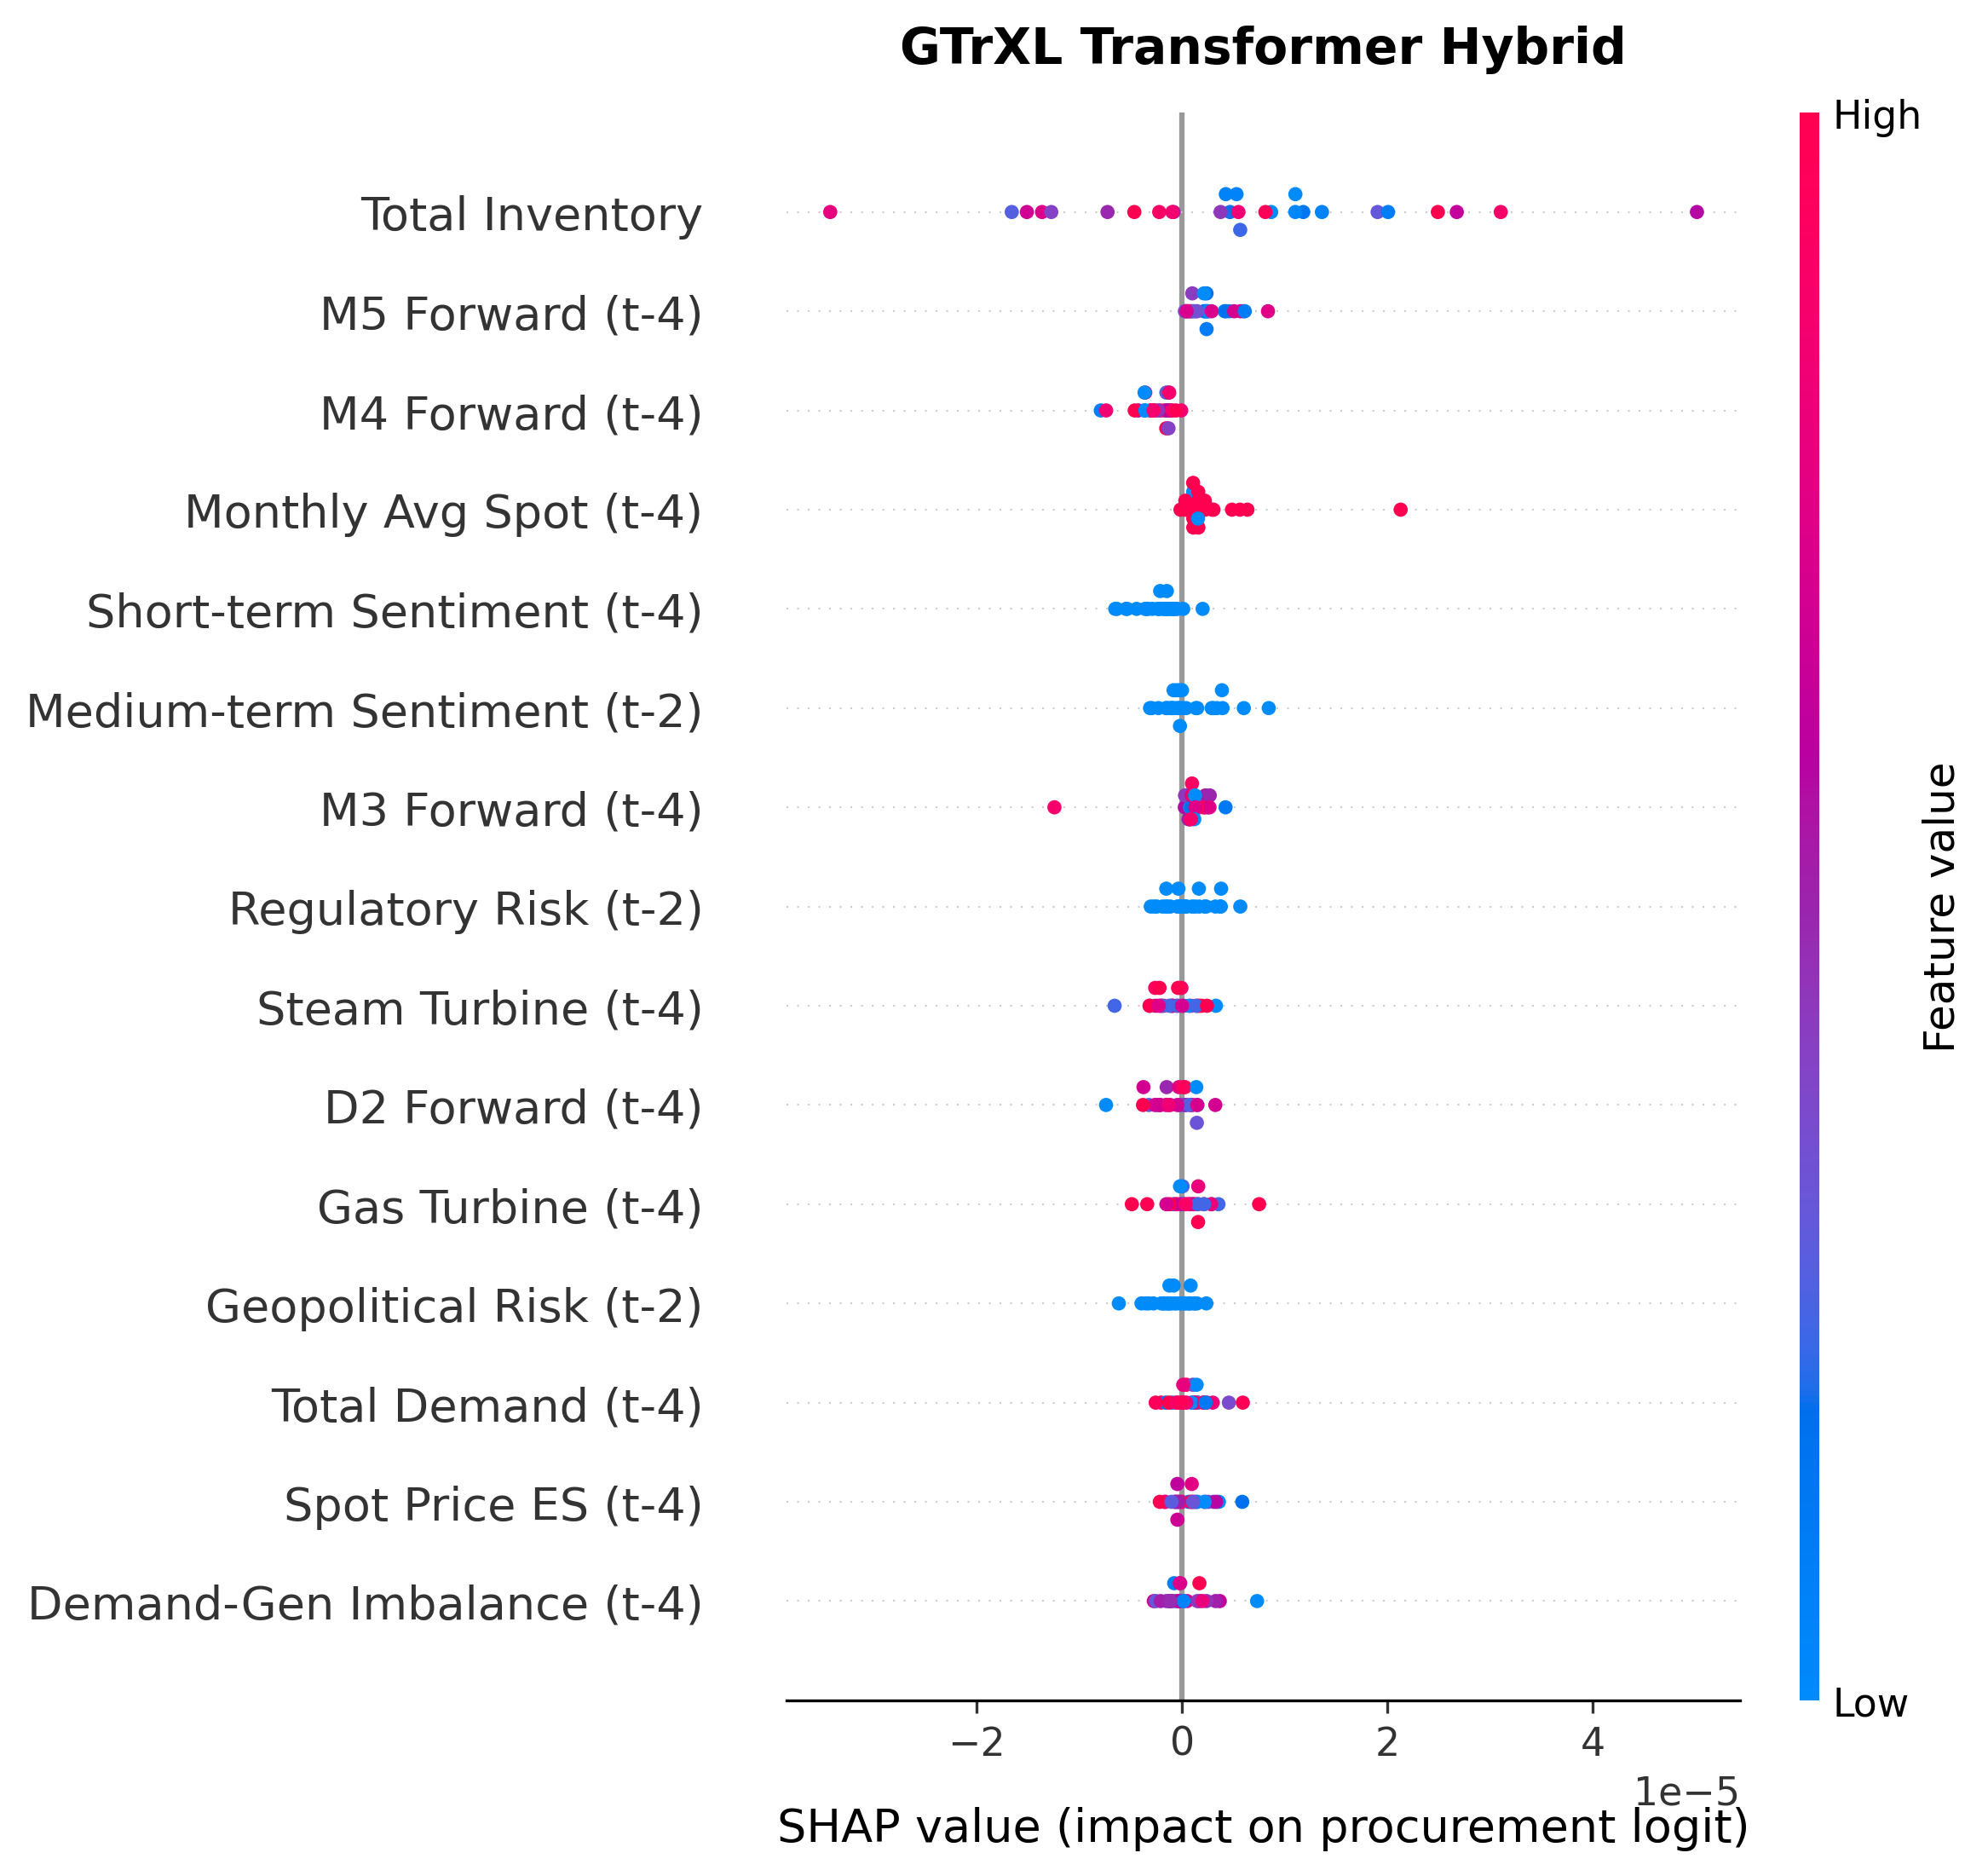
\includegraphics[width=\textwidth]{fig11_shap_transformer_hibrido.png}
        \caption{GTrXL Transformer Hybrid}
        \label{subfig:shap_gtrxl_hybrid}
    \end{subfigure}
    \hfill
    \begin{subfigure}[b]{0.48\textwidth}
        \centering
        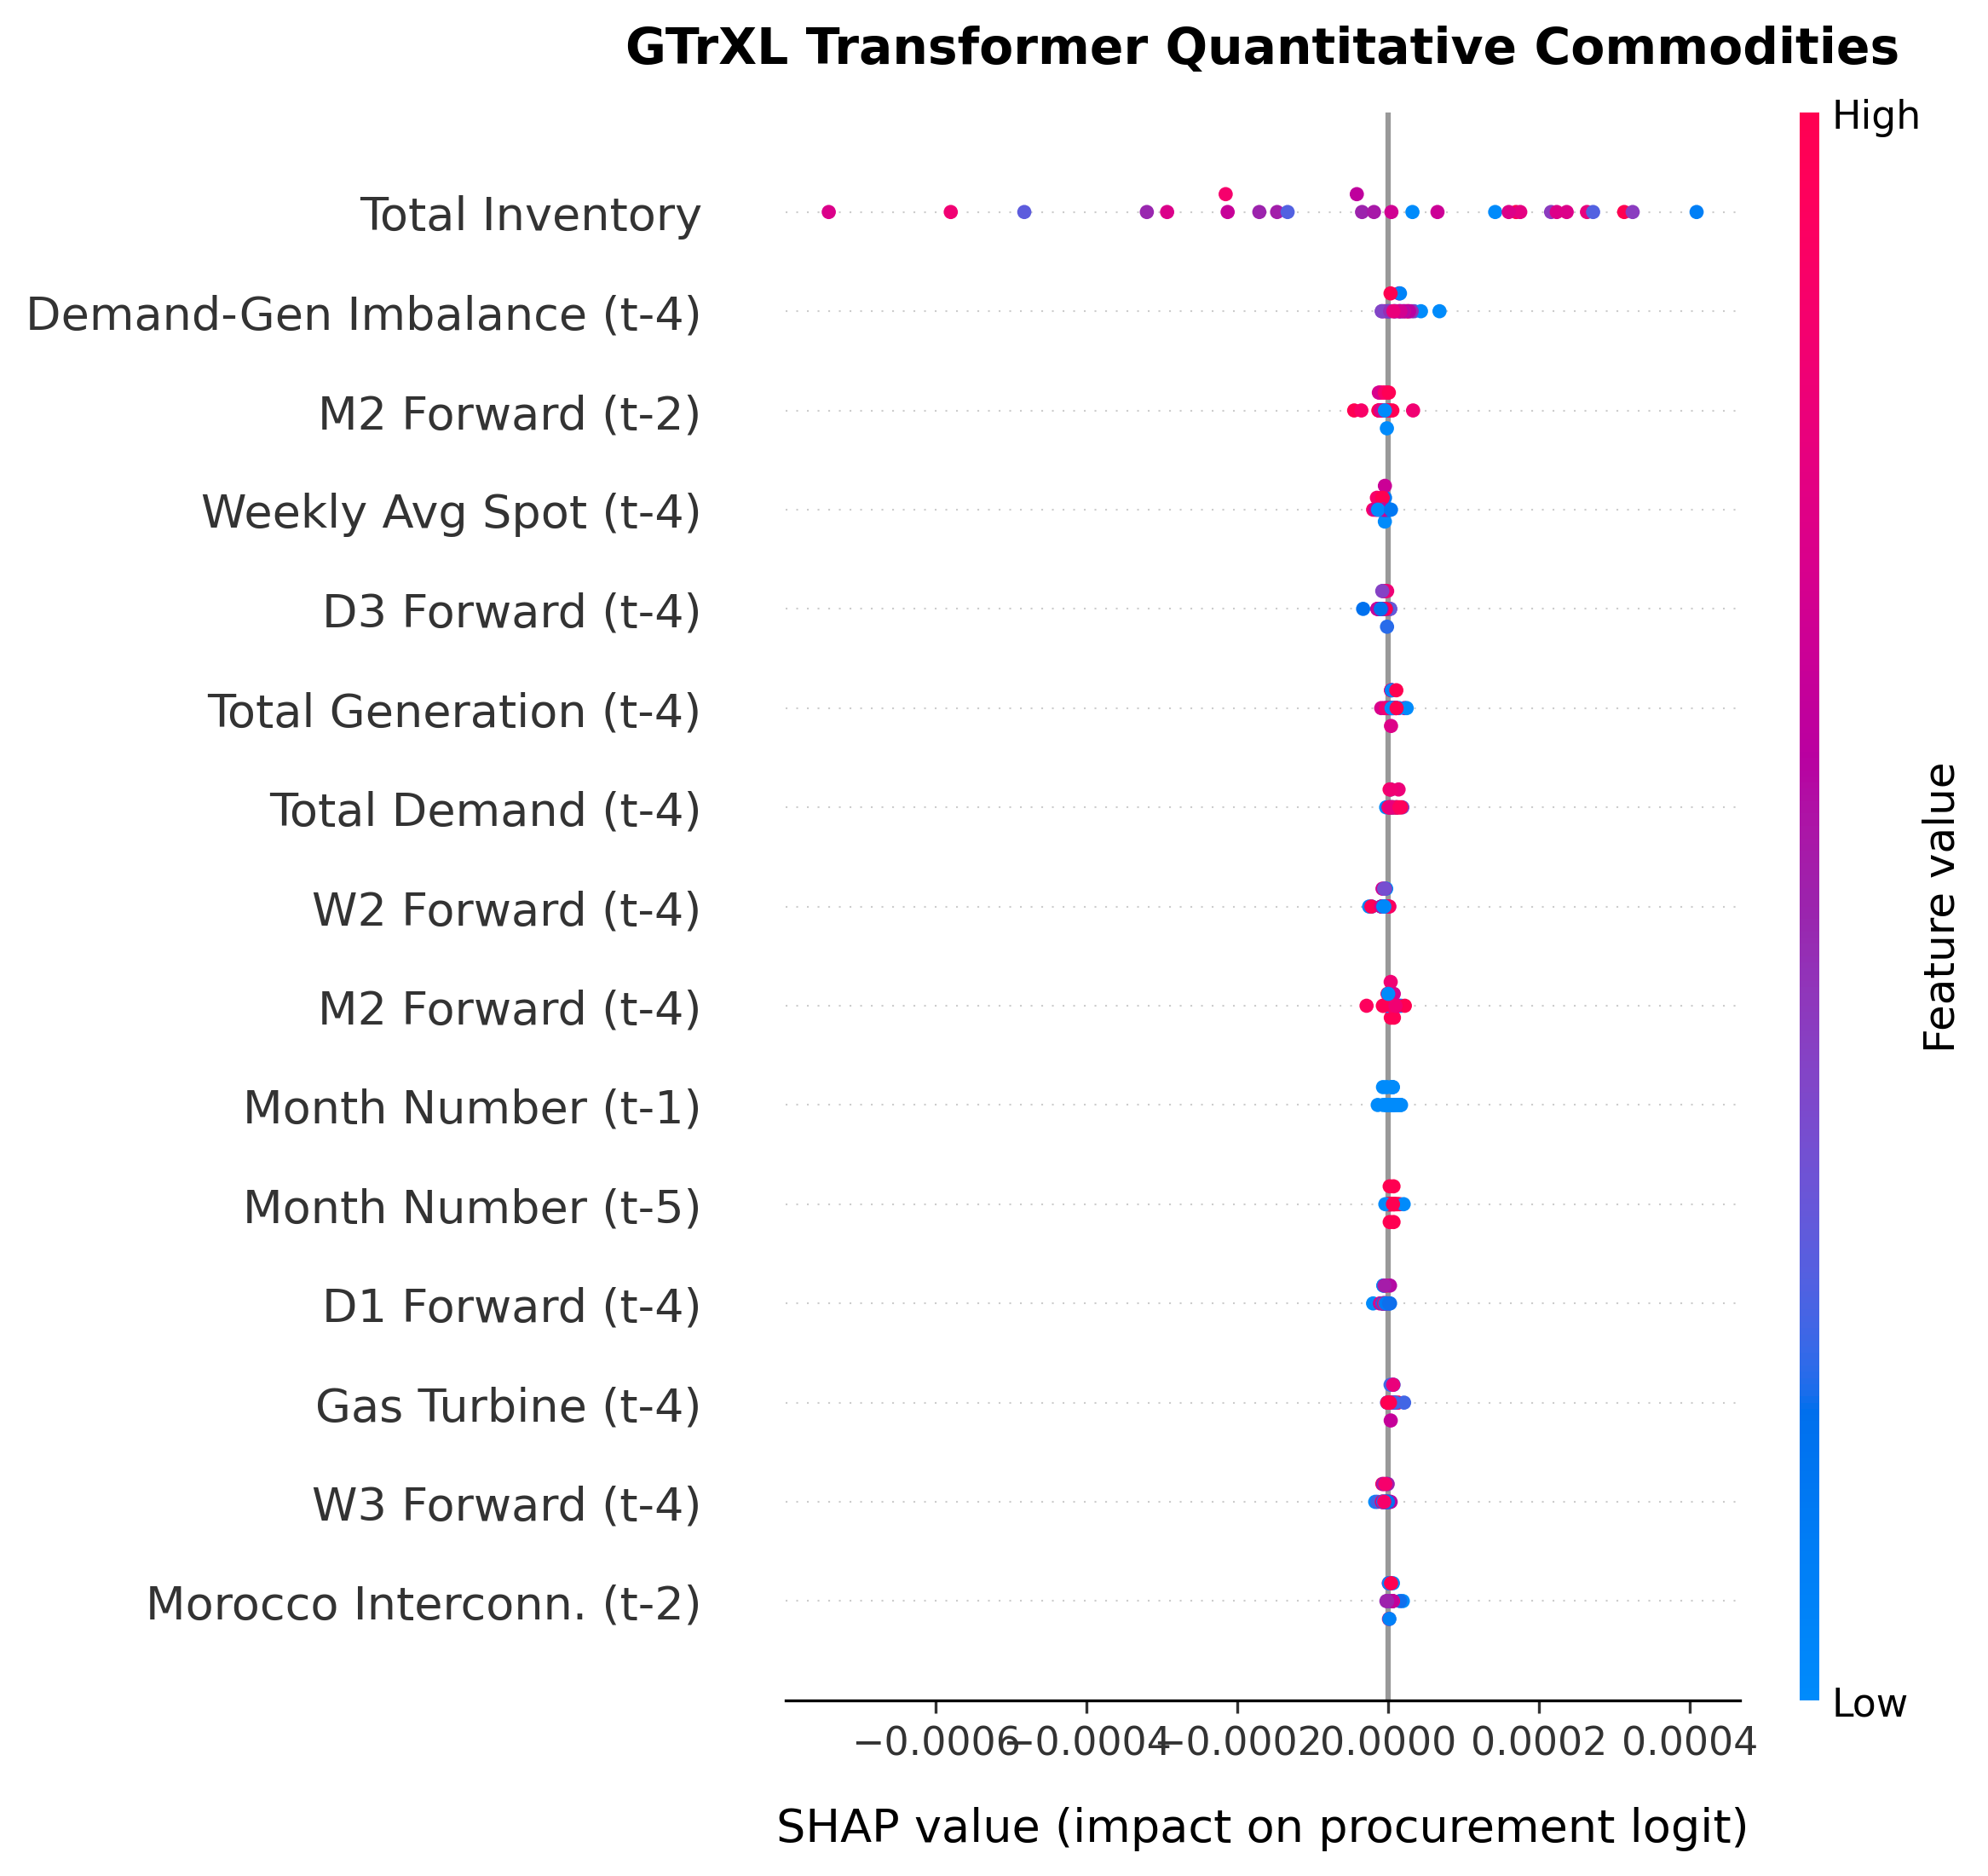
\includegraphics[width=\textwidth]{fig11_shap_transformer_fisico.png}
        \caption{GTrXL Transformer Quantitative Commodities}
        \label{subfig:shap_gtrxl_physical}
    \end{subfigure}
    \vskip\baselineskip
    \begin{subfigure}[b]{0.48\textwidth}
        \centering
        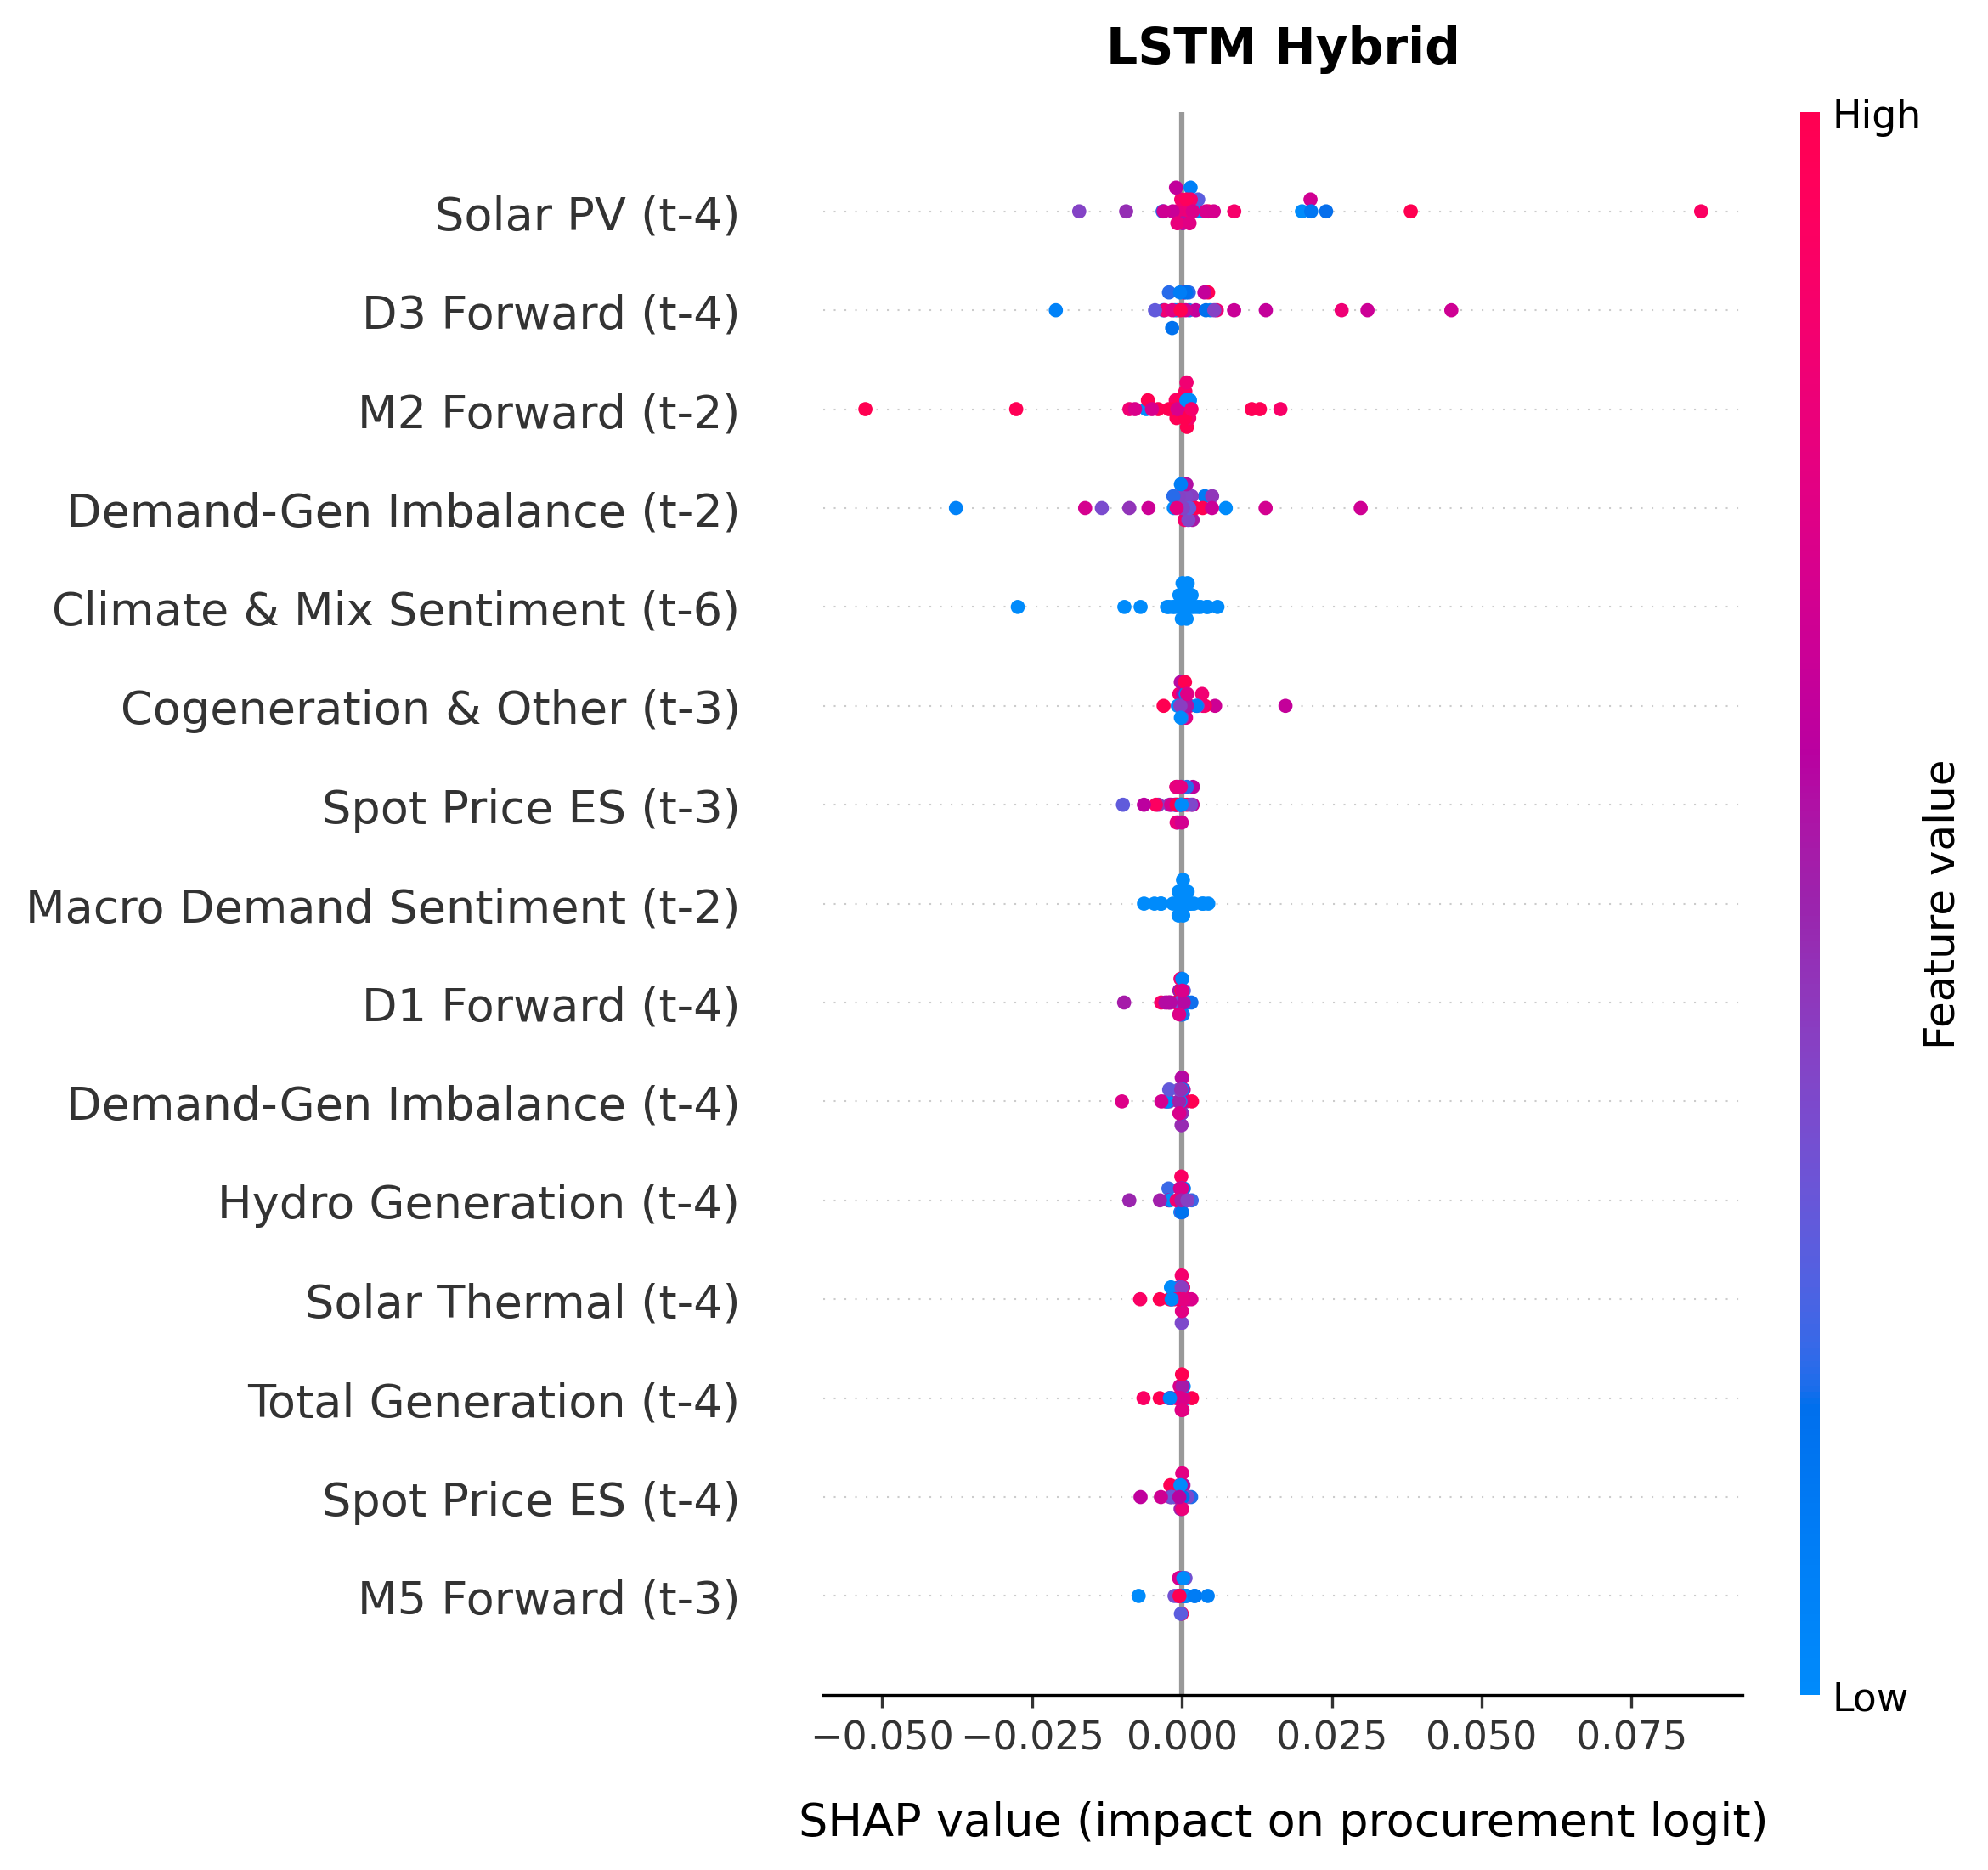
\includegraphics[width=\textwidth]{fig11_shap_lstm_hibrido.png}
        \caption{LSTM Hybrid}
        \label{subfig:shap_lstm_hybrid}
    \end{subfigure}
    \hfill
    \begin{subfigure}[b]{0.48\textwidth}
        \centering
        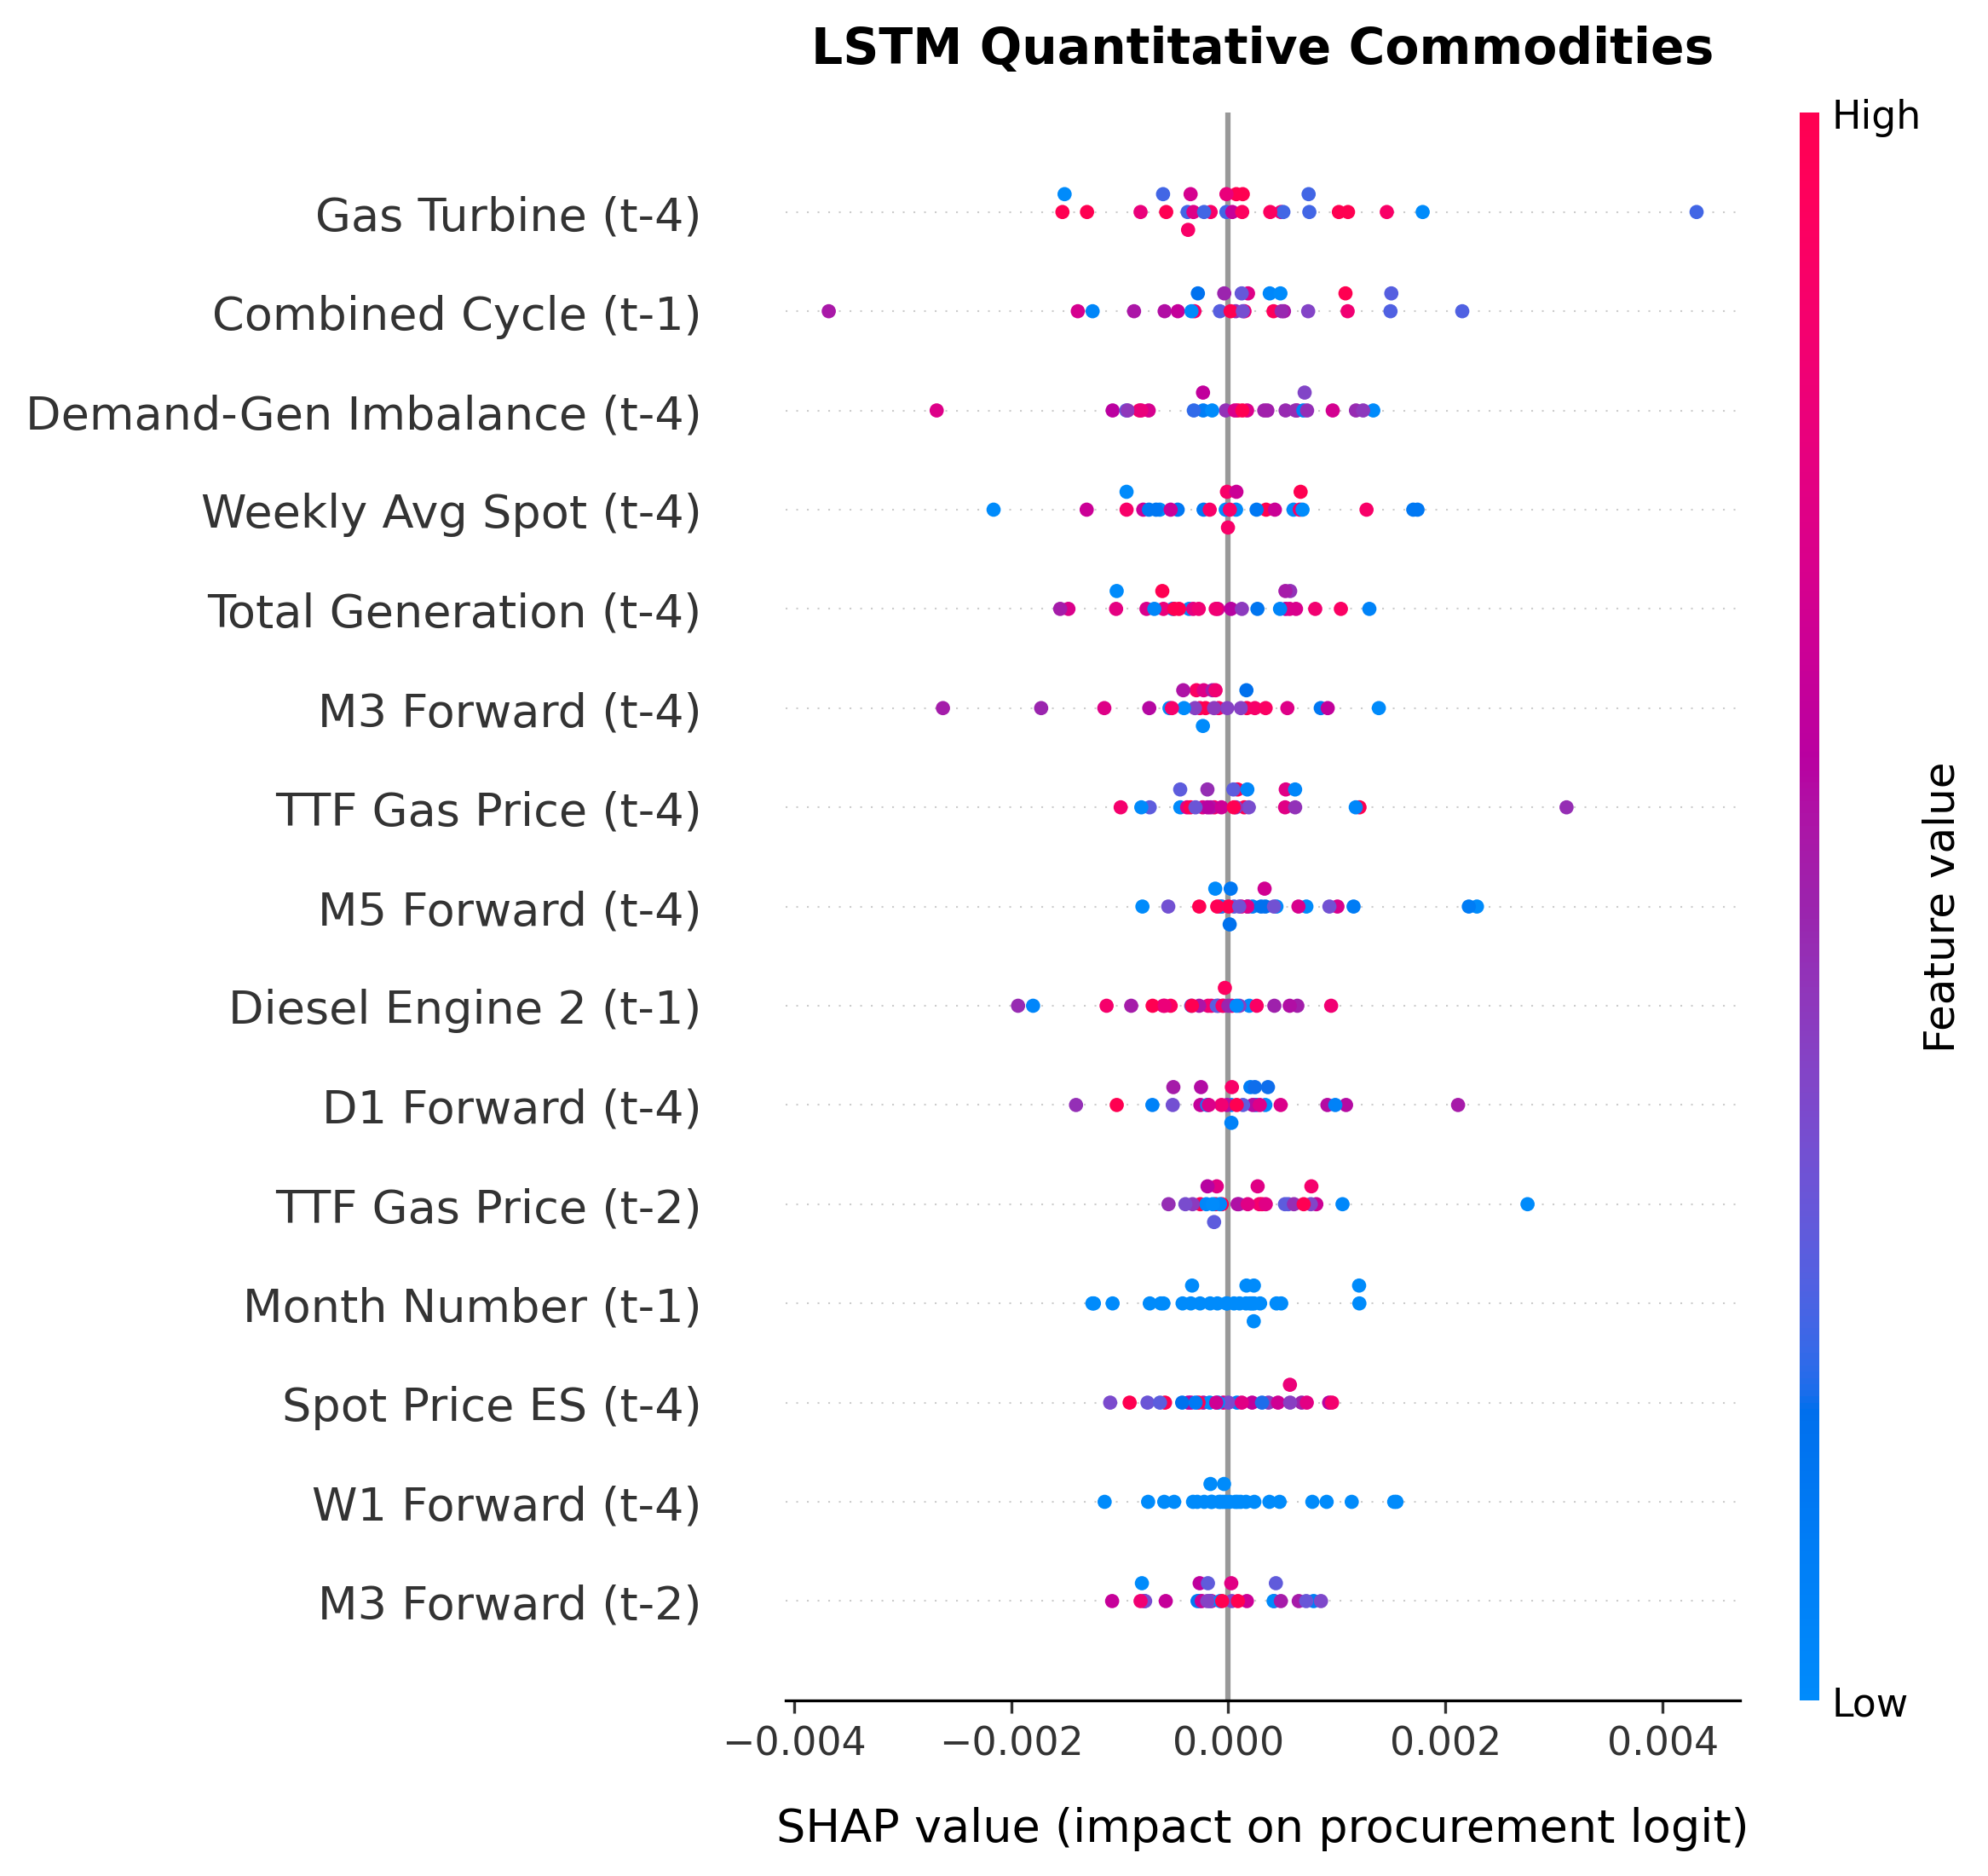
\includegraphics[width=\textwidth]{fig11_shap_lstm_fisico.png}
        \caption{LSTM Quantitative Commodities}
        \label{subfig:shap_lstm_physical}
    \end{subfigure}
    \caption{SHAP feature attribution summary across 2026 evaluation observations for Phase~4 models. Points represent daily observations colored by feature value (red: high, blue: low); horizontal dispersion reflects directional impact on policy procurement logits.}
    \label{fig:shap_comparison}
\end{figure*}

The attribution profiles in \cref{fig:shap_comparison} reveal distinct structural patterns across the evaluated configurations. In the GTrXL Hybrid model (\cref{subfig:shap_gtrxl_hybrid}), aggregated forward commitment inventory features yield the largest mean absolute SHAP magnitude among evaluated predictors (mean absolute SHAP $= 1.33 \times 10^{-5}$), showing that existing forward commitments strongly govern policy decisions. Furthermore, text-derived sentiment dimensions rank within the top 15 most influential predictors in the hybrid architectures. While the full observation vector comprises $\text{dim}(\mathbf{o}_t) = 715$ dimensions, the SHAP gradient explainer is computed over the 318 active input dimensions that exhibit non-zero gradient variance: 31 dynamic market features across $L=7$ historical lookback lags ($31 \times 7 = 217$ inputs) plus the first 101 forward inventory delivery offsets ($h \in \{1, \dots, 101\}$ days). As an empirical finding, the trained policies never selected long-horizon forward contracts ($M_4$--$M_6$), leaving delivery offsets $h > 101$ days at zero allocation ($m_t(h)=0$) with constant sentinel values $-10.0$ and identically zero gradients. Specifically, short-term sentiment (\texttt{Short-term Sentiment}, rank 6), medium-term sentiment (\texttt{Medium-term Sentiment}, rank 7), regulatory intervention risk (\texttt{Regulatory Intervention Risk}, rank 9), and geopolitical risk (\texttt{Geopolitical Risk}, rank 13) exhibit high attribution magnitude, with heightened geopolitical risk scores systematically associated with elevated logits for short-horizon forward contracts ($D_2/D_3$). In contrast, for the LSTM Hybrid model (\cref{subfig:shap_lstm_hybrid}), physical grid coupling variables---most notably solar PV generation (\texttt{Solar PV}) and the generation-demand imbalance (\texttt{Generation-Demand Imbalance})---dominate the highest attribution ranks alongside forward contract quotes ($D_3$, $M_2$), while climate and generation mix sentiment (\texttt{Climate \& Mix Sentiment}, rank 6) and macroeconomic demand sentiment (\texttt{Macroeconomic Demand}, rank 9) receive non-negligible attribution.

These attribution results describe empirical associations between input features and policy outputs within the evaluated sample conditioned on the lookback window and $h_0 = \mathbf{0}$. We emphasize that SHAP attributions reflect internal directional associations between input gradients and policy logits in the fitted Phase~4 models (whose architecture hyperparameters were tuned across the full horizon). Consequently, these feature attributions describe the internal decision logic of the post-selection network rather than providing an independent validation of semantic construct validity, proving a structural causal relationship between news sentiment and forward price dynamics, or demonstrating that the agent explicitly forecasts market price collapses. The near-zero attribution assigned to distant collinear indicators is consistent with effective representation filtering on local observation gradients, focusing policy sensitivity on high-relevance physical balances and regulatory sentiment while attenuating redundant market signals within the evaluated state space.
